% Relatório SBC · Análise de redes de transporte público de Belo Horizonte
%
% Estrutura e orçamento de páginas: docs/fontes/plano-de-projeto.md §14.1.
% Uma seção por arquivo em secoes/; cada dono edita só os arquivos da sua seção.
% Seção de feature: crie secoes/<ID>.tex (ex.: secoes/F-ROTA.tex); ela entra sozinha
% em secoes/funcionalidades.tex. Figuras em figuras/.
% Compilar: ver relatorio/README.md. Limite: 12 a 15 páginas.

\documentclass[12pt]{article}

\usepackage[T1]{fontenc}
\usepackage[utf8]{inputenc}
\usepackage[brazilian]{babel}
\usepackage{sbc-template}
\usepackage{graphicx}
\usepackage{url}
\usepackage{amsmath,amssymb}
\usepackage{booktabs}
\usepackage{tabularx}
\usepackage{xcolor}

\graphicspath{{figuras/}}

% Texto ainda não escrito. Sai em cinza no PDF para ninguém esquecer; some quando a
% seção é escrita. Nenhuma versão entregue pode conter \pendente.
\newcommand{\pendente}[1]{{\color{gray}\itshape[#1]}}

% Inclui secoes/<ID>.tex se existir; senão, mostra o aviso (essenciais) ou nada.
\newcommand{\secaofeature}[2]{%
  \InputIfFileExists{secoes/#1}{}{\subsection{#2}\pendente{#1 ainda sem seção: criar secoes/#1.tex}}}
\newcommand{\secaofeatureopcional}[1]{\InputIfFileExists{secoes/#1}{}{}}

\sloppy

\title{Análise de redes de transporte público de Belo Horizonte\\com grafos}

\author{Thiago\inst{1}, Miguel\inst{1}, Henrique\inst{1}, Arthur\inst{1}, Caio\inst{1}, Rafael\inst{1}}

\address{\pendente{curso, instituição e cidade}
  \email{\pendente{e-mails}}
}

\begin{document}

\maketitle

\begin{abstract}
  \pendente{Abstract em inglês, até 10 linhas, escrito por último (Rafael, P3).}
\end{abstract}

\begin{resumo}
  \pendente{Resumo em português, até 10 linhas, escrito por último (Rafael, P3).}
\end{resumo}

% Seção: Introdução
% Dono: Henrique · Orçamento: 1 página(s) · docs/fontes/plano-de-projeto.md §14.1
% Conteúdo: Contexto, problema, objetivos e as seis perguntas
\section{Introdução}\label{sec:intro}

\pendente{Contexto, problema, objetivos e as seis perguntas. Dono: Henrique.}

% Seção: Fundamentação
% Dono: Thiago e Henrique · Orçamento: 1 página(s) · docs/fontes/plano-de-projeto.md §14.1
% Conteúdo: GTFS, modelos de grafo para transporte, algoritmos usados
\section{Fundamentação}\label{sec:fund}

\pendente{GTFS, modelos de grafo para transporte, algoritmos usados. Dono: Thiago e Henrique.}

% Seção: Dados
% Dono: Miguel · Orçamento: 1 página(s) · docs/fontes/plano-de-projeto.md §14.1
% Conteúdo: Fonte, limpeza, recorte e estatísticas da rede
\section{Dados}\label{sec:dados}

O projeto usa o GTFS convencional publicado pela Prefeitura de Belo Horizonte
(\url{https://dados.pbh.gov.br/dataset/gtfs}). O instantâneo baixado em 05/11/2026
foi identificado pelo SHA-256 iniciado em \texttt{623bdf422fb0}; o valor
completo está no arquivo da feature P0-DADOS.
O script de download registra origem e data fora do Git para permitir reproduzir
as medições com o mesmo arquivo.

O leitor converte paradas, linhas, viagens, horários e calendário em uma rede
normalizada. Seleciona uma quarta-feira ativa, aplica as exceções de
\texttt{calendar\_dates.txt}, conserva os horários por viagem e relata linhas
inválidas. A leitura de \texttt{stop\_times.txt} é feita em fluxo. Um recorte por
caixa geográfica ou linhas preserva apenas trechos consecutivos, sem criar uma
ligação direta onde uma parada intermediária foi removida. A
Figura~\ref{fig:atividade-dados} resume o processamento.

\begin{figure}[ht]
  \centering
  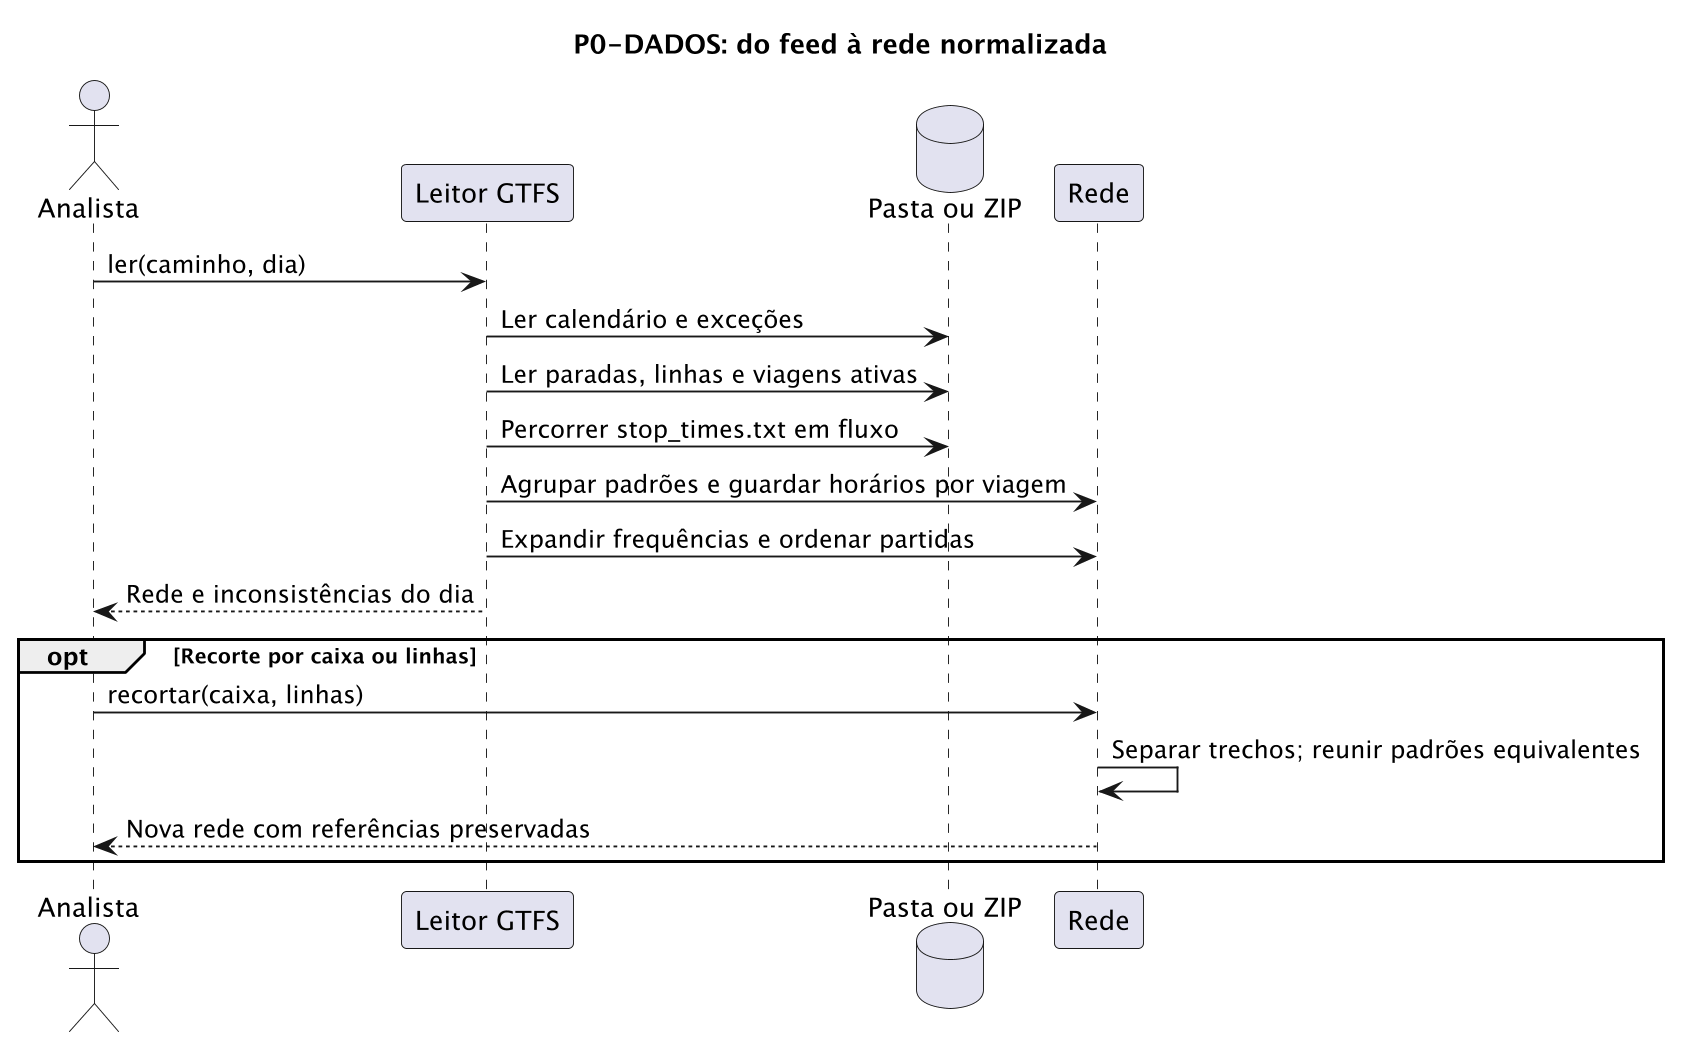
\includegraphics[width=0.82\linewidth]{sequencia-dados-resumo.png}
  \caption{Leitura e recorte do GTFS até a rede normalizada.}
  \label{fig:atividade-dados}
\end{figure}

No serviço de 04/11/2026, a execução de \texttt{ler("dados/brutos/bhtrans.zip")}
produziu 9.659 paradas, 303 linhas, 698 padrões e 24.503 viagens. O leitor não
reportou inconsistências para esse serviço. A leitura foi medida com
\texttt{medir(ler, caminho, repeticoes=3)}: média de 7,753~s e desvio amostral
de 0,114~s em MacBook Air com Apple M4, 16~GB e Python~3.14.6. Esses valores
descrevem o modelo de dados; o número de arestas só existe após construir uma
visão de grafo. A validação atual examina o dia selecionado, não todas as datas
de vigência do feed.

% Seção: Modelagem
% Dono: Henrique · Orçamento: 2,5 página(s) · docs/fontes/plano-de-projeto.md §14.1
% Conteúdo: Modelo de dados, visões G_P, G_E, G_L e G_T, diagramas UML
\section{Modelagem}\label{sec:modelagem}

\pendente{Modelo de dados, visões $G_P$, $G_E$, $G_L$ e $G_T$, diagramas UML. Dono: Henrique.}

% Seção: Plano de desenvolvimento
% Dono: Henrique · Orçamento: 0,5 página(s) · docs/fontes/plano-de-projeto.md §14.1
% Conteúdo: Método, divisão e calendário (Etapa 1)
\section{Plano de desenvolvimento}\label{sec:plano}

\pendente{Método, divisão e calendário (Etapa 1). Dono: Henrique.}

% Seção: Implementação
% Dono: Thiago e Arthur · Orçamento: 1 página(s) · docs/fontes/plano-de-projeto.md §14.1
% Conteúdo: Núcleo de grafo e heap, organização do código e interface
\section{Implementação}\label{sec:impl}

\pendente{Núcleo de grafo e heap, organização do código e interface. Dono: Thiago e Arthur.}

% Seção: Funcionalidades e resultados
% Dono: cada dono de feature · Orçamento: 4 páginas no total · plano-de-projeto §14.1
% Conteúdo: uma subseção por feature, com tela, resultado e complexidade.
%
% Como encaixar a sua feature: crie relatorio/secoes/<ID>.tex começando com
% \subsection{<título>}\label{sec:<ID>}. Ela entra aqui sozinha, sem editar este arquivo.
% Essenciais mostram um aviso enquanto o arquivo não existir; desejáveis e opcionais
% só aparecem quando o arquivo existir.
% Cada subseção traz: figura (tela), resultado com o número medido, complexidade e
% uma limitação. Nenhum número sem execução real (AGENTS.md §5, regra 6).
\section{Funcionalidades e resultados}\label{sec:funcionalidades}

% Essenciais (P1)
\secaofeature{F-ROTA}{Trajeto mais rápido}
\secaofeature{F-ESPERA}{Espera e simulação de trajeto}
\secaofeature{F-BALD}{Menos baldeações}
\secaofeature{F-MET}{Centralidades}
\secaofeature{F-EFI}{Eficiência da rede}
\secaofeature{F-RES}{Falhas e resiliência}

% Desejáveis (P2)
\secaofeatureopcional{F-ROTA-2}
\secaofeatureopcional{F-ESPERA-2}
\secaofeatureopcional{F-BALD-2}
\secaofeatureopcional{F-MET-2}
\secaofeatureopcional{F-EFI-2}
\secaofeatureopcional{F-RES-2}

% Opcionais
\secaofeatureopcional{F-ROTA-OPC}
\secaofeatureopcional{F-ESPERA-OPC}
\secaofeatureopcional{F-BALD-OPC}
\secaofeatureopcional{F-MET-OPC}
\secaofeatureopcional{F-EFI-OPC}
\secaofeatureopcional{F-RES-OPC}

% Seção: Avaliação de desempenho
% Dono: Rafael · Orçamento: 1 página · docs/fontes/plano-de-projeto.md §14.1
% Conteúdo: complexidade teórica e tempos medidos de cada algoritmo; comparação com
% NetworkX só se a etapa opcional (F-AVAL-OPC) acontecer.
% A tabela é preenchida na F-AVAL (RF-AVA-02) com os números registrados nos arquivos
% de feature. Nenhum número entra aqui sem o comando que o gerou.
\section{Avaliação de desempenho}\label{sec:avaliacao}

\subsection{Metodologia de medição}

Todos os tempos deste relatório foram obtidos com a mesma função,
\texttt{medir}, do módulo \texttt{transporte.util.medicao}. Ela executa o
algoritmo $N$ vezes com os mesmos argumentos (por padrão, $N = 5$) e
cronometra cada execução isoladamente com \texttt{time.perf\_counter}, o
relógio monotônico de maior resolução do Python~\cite{python-perf-counter}.
Só a chamada do algoritmo fica dentro do intervalo medido: a leitura do GTFS e
a construção do grafo são medidas à parte, quando interessam. O resultado é a
média $\bar{t}$ e o desvio padrão amostral
\[
  s = \sqrt{\frac{1}{N-1}\sum_{i=1}^{N}(t_i - \bar{t})^2},
\]
com divisor $N - 1$ porque as $N$ execuções são uma amostra do tempo do
algoritmo naquela máquina, e não a população inteira. Com $N = 1$, o desvio é
reportado como zero.

Cada tempo é acompanhado do tamanho do grafo ($|V|$ e $|E|$ da visão usada) e
da máquina em que foi medido, porque tempo de parede só é comparável dentro da
mesma máquina e da mesma rede. A complexidade teórica de cada algoritmo vem da
docstring da função correspondente, justificada no arquivo da feature.

\subsection{Complexidade e tempos medidos}

\pendente{Tabela consolidada (F-AVAL, RF-AVA-02): algoritmo, visão, complexidade
teórica, $|V|$, $|E|$, tempo médio $\pm$ desvio e $N$, com os números
registrados por cada dono na rede real.}

\subsection{Comparação com o NetworkX}

\pendente{Só se a etapa opcional F-AVAL-OPC acontecer (16/11 a 18/11); caso
contrário, esta subseção sai.}

% Seção: Limitações e conclusão
% Dono: Caio · Orçamento: 1 página(s) · docs/fontes/plano-de-projeto.md §14.1
% Conteúdo: O que o modelo não captura e o que fica para depois
\section{Limitações e conclusão}\label{sec:conclusao}

\pendente{O que o modelo não captura e o que fica para depois. Dono: Caio.}

% Seção: Responsabilidades
% Dono: Rafael · Orçamento: 0,5 página · docs/fontes/plano-de-projeto.md §14.1
% Conteúdo: quem fez o quê, a partir da tabela-mestre
% (docs/plano-de-desenvolvimento/README.md) e do git log.
% v1 (03/11): divisão planejada. No P3, confirmar com o git log e com as features que de
% fato fecharam o Definition of Done; o que saiu do escopo sai da tabela.
\section{Responsabilidades}\label{sec:responsabilidades}

A Tabela~\ref{tab:responsabilidades} resume a divisão do trabalho. Cada
integrante foi dono de uma frente: a fundação de uma área do código e as
funcionalidades que a estendem.

\begin{table}[ht]
\centering
\caption{Divisão do trabalho entre os integrantes.}
\label{tab:responsabilidades}
\footnotesize
\begin{tabularx}{\textwidth}{@{}l>{\raggedright\arraybackslash}X>{\raggedright\arraybackslash}X@{}}
\toprule
Integrante & Fundação e integração & Funcionalidades \\
\midrule
Thiago   & Núcleo de grafos, heap e buscas & Centralidades \\
Miguel   & Leitura do GTFS, modelo normalizado e rede de teste & Espera e simulação de trajeto \\
Henrique & Modelagem, diagramas UML e construtores das visões & Trajeto mais rápido \\
Arthur   & Aplicação Streamlit e componente de mapa & Eficiência da rede \\
Caio     & Repositório, verificação de imports e guia do projeto & Falhas e resiliência \\
Rafael   & Relatório e medição de tempo & Menos baldeações; avaliação de desempenho \\
\bottomrule
\end{tabularx}
\end{table}

\pendente{P3: acrescentar as desejáveis e opcionais que foram concluídas e conferir
com o \texttt{git log}.}


\bibliographystyle{sbc}
\bibliography{referencias}

\end{document}
